\documentclass[12pt]{article}
\usepackage{fullpage}
\usepackage{nopageno}
\usepackage{ifthen}
\usepackage{amsmath}
\usepackage{amssymb}
\usepackage{graphicx} 
%\usepackage{add-copyright}

\newcommand{\R}{\mathbb{R}}

\title{Take-Home Quiz 3}
\author{Math 131 Section 22}
\date{Due Monday, October 31, 2005}

\newcounter{problem}
\setcounter{problem}{1}

\newenvironment{problem}[1][]
{\begin{flushleft}\hangindent=1em\hangafter=1\noindent\textbf{Problem \arabic{problem}.}
\ifthenelse{\equal{#1}{}}{}{
\textbf{(#1 \ifthenelse{\equal{#1}{1}}{point}{points}).}}
}
{\addtocounter{problem}{1}\end{flushleft}}

\begin{document}
\maketitle

\begin{problem}[3]
Let $f : \R \to \R$ be a differentiable function.  Prove $f$ is continuous.
\end{problem}

\vfill

\begin{problem}[3]
Give an example of a continuous function $f : \R \to \R$ which is
differentiable on $(-\infty,0) \cup (0,1) \cup (1,\infty)$ but fails
to be differentiable at $0$ and $1$.
\end{problem}

\vfill

\pagebreak

\begin{problem}[3]
Define $f : \R \to \R$ by $f(x) = 2x - x^2$.  Prove, using the
definition of derivative, that $f'(x) = 2 - 2x$.
\end{problem}

\vfill

\begin{problem}[2]
Sketch the derivative of the left-hand graph on the empty right-hand graph.
\begin{center}
\includegraphics[angle=-90,width=3in]{squared-graph.ps}
\hfill
\includegraphics[angle=-90,width=3in]{empty-graph.ps}
\end{center}
\end{problem}

\vspace{2ex}

\begin{problem}[2]
Sketch the derivative of the left-hand graph on the empty right-hand graph.
\begin{center}
\includegraphics[angle=-90,width=3in]{weird-graph.ps}
\hfill
\includegraphics[angle=-90,width=3in]{empty-graph.ps}
\end{center}
\end{problem}




\end{document}
